\section{Historical Perspective}


Throughout the 80's and 90's, the increasing demand for performance was met by
increasing the clock frequency. Shortening the critical path and exploiting
instruction level parallelism allowed the CPU to run at higher clock speeds to
improve performance \cite{tanenbaum1984structured}. Consequently, processor
manufacturers were able to double single-threaded performance approximately
every 18th month \cite{moore1965cramming}. The tradeoff, however, was an
increased amount of complex logic added complexity to the processor core.
Greater complexity required a greater amount of transistors which must fit on
the same die, made possible by the reduction of transistor size. For a long
time, new process technologies allowed for smaller and less energy consuming
transistors, but as we approached the end of Dennard scaling
\cite{dennard1974design,esmaeilzadeh2011dark}, the amount of logic required to
accomodate speedups could not fit on the die due to thermal constraints. Heat
generation on-chip became overwhelming and one could not simply increase the
frequency or add extra logic to gain additional performance.

\begin{figure}
    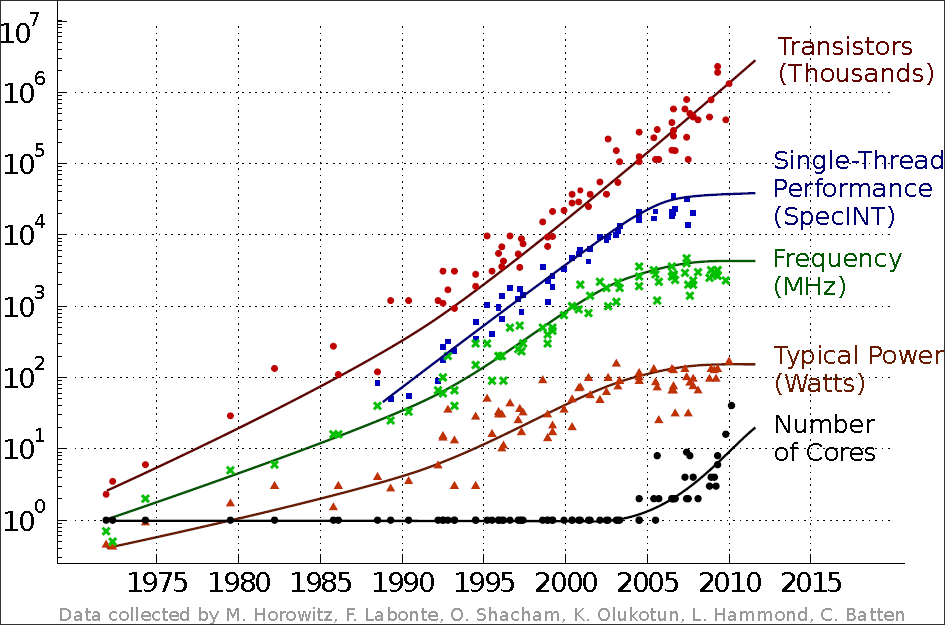
\includegraphics[width=\textwidth]{figs/cpu-performance.png}
    \caption{Historical trends in CPU performance, from \cite{salishan2011}}
    \label{fig:cpuperformance}
\end{figure}

The tremendous growth in performance is depicted in
\autoref{fig:cpuperformance}. We note that although the transistor count is
steadily increasing, single-threaded performance has only seen a minor increase
the last few years.




